\chapter{Towards a metabolic theory of biogeography}
\label{chap4}


\subsection{Résumé en français du troisième article}

Dpeuis longtems cotrinate énergétqies
En 2015 j'ai comencà à m'interessé au problème energie mais pa assez et puis j'ai commencé

Cet article présente d'une extension du modèle de la TTIB \citep{Gravel2011}
que je proposed de reformuler en terme de contrainte énergétiques.


des reflexiosn pour lever le nombre d'espèce dans mon modèle mais aussi à essayer d'aller vers qulqueauchose qui est plus réalistes.
Quand on pense à une pyramide du viavant uil y a la base des producitoeru qui de l'energie inogranique jusqu'au top prédateurs sont capables de faire de l'énergie.
COmme souligné par le pepier de gravel et al. il n'y a le simple fat qu'un prédateur mais aussi il y a une différenece de triantemnt dansun top prédateur et un herbivore dans la rpartitoin de l'énergie. J'ai essayeé de me vconfrointer à ces porblèmes mais j'ai du commencé par comprendre l'.tat du svaoir et les enjeux. Il m'apparait que 2 théories int.ressantes plus ou moins mécanistqieu amais pas tant de pronlèeme. Mais comment comprendre que certain relation soit visibles à lare échelle est difficile à comprendre ou sont la preuve que certaine hypothèse nitamen la saturation..
Ce modèle offre des perspectives nouvelles et un point d'ancrage concret sur plein de belles choses.



\subsection{Publication envisagée}

En l'état plutot théorique et lève un certains nombre d'obstacle en ce sens
mais aussi aller plus loin avec des données en post doc et aussi plu loind ans population
proposée pour post doc... 

Ce article traite de deux ascpect les perspectives qu'offre un approche et propose un proeneir pas pour sclaer ver sles ppulations depuis le haut.
Le modèle qui y est présenté est simple mais innovant et offre possibilité pour explorer des hypothèses.
Le chapitre est en cours de dévelpppement. L'avancement est indiqué dans le rapport du troisième compte-rendu de comité de thèse.
Il est la base d'un porjet que je viens de proposer pour le post doc.
Miguel Araujo et Loic Pelissier. cool

Un grand merci à Solraik..
\section{Introduction}\label{introduction}

Disentangling the respective contribution of processes shaping species
distribution remains the central principle of biogeography. While
biogeographers clearly envision the list of ingredients that are needed
to understand species distribution \citep{Thuiller2013}, they are
currently lacking an ideal recipe, which has the right individual
proportions toward forecasting accurately community assembly. Therefore,
in the current context of global changes, we likely fail to predict
accurately biodiversity responses as we keep our focus strictly on
abiotic factors \emph{i.e} temperature and precipitation, while
continuing to overlooking biotic interactions and short-term
evolutionary responses \citep{Lavergne2010}. At the core of this issue
is the need for a renewal of theoretical foundations that currently
exist in the field of biogeography, which should be started by a
synthesis of recent enrichments of the model of the island-based theory
of biogeography \citep{Lomolino2000a, Warren2015}.

Among major theoretical challenges toward more realistic models, biotic
interactions should be integrated as a constraint for species
co-existence in meta-communities \citep{Jabot2012, Cazelles2015a}.
Community ecology involves the interplay of species together, where they
interact and their persistence within the community relies heavily on
their relationships. Consequently, ecological interactions may explain,
at least partially, the dynamics of local extinctions, which in turn
would further explain some properties of the geometrical shape of the
ranges of species \citep[\emph{e.g.} nested distributions of parasitoid
and its host,][]{Shenbrot2007t} even if we have poor evidence of such
effect at large spatial scales \citep[but see][]{Gotelli2010}. However,
two of the most influential models in biogeography assume ecological
equivalence of species; the Theory of Island Biogeography of MacArthur
and Wilson \citep[hereafter TIB,][]{MacArthur1967}, which consistently
overlook the variation among species characteristics, especially when
considering their interactions within food-webs. Second, in his neutral
theory, Hubbell assumes that individuals of different species are
ecologically equivalent and predicts the distribution of abundance
without considering interactions \citep{Hubbell1997}. These two
theoretical models have been proven relevant for certain groups of
species and inadequate for others, but none of them were initially
intended to describe exhaustively the different components of
communities on islands. To make strides towards increased predictive
power at the community scale, the hypothesis of ecological equivalence
must be released and ecological interactions explicitly integrated
\citep{Holt2010, Gravel2011}.

The TIB is well-suited to explore the consequences of the integration of
ecological interactions at broad spatial scales as it includes two
fundamental processes of biogeography, immigration and extinction in an
elegant fashion that eases its extension \citep{Losos2010, Warren2015}.
Building upon the classical models, recent studies have included
interactions in the TIB \citep{Gravel2011, Cazelles2015a}. In such
approaches, the regional pool of speciesl becomes a \emph{metaweb} which
makes species inter-dependent entities with specificities (\emph{e.g.} a
given trophic level) rather than indistinguishable unities of a species
quantity allowing so more than the prediction of species richness
\citep[\emph{e.g} the occurrence probabilities of species from different
trophic levels][]{Gravel2011}. As an important consequence of such
consideration, colonization and extinction rates vary with respect to
the species identity and the local community. \citet{Gravel2011}
proposed that Trophic TIB (hereinafter TTIB), where predators can
survive locally just as long as they find at least one prey and prevent
their colonization if for prey-free islands. More generally,
\citet{Cazelles2015} presented a Lotka-Volterra like model in which the
composition of the local community determines the extinction rates.
Despite the increase of the realism of the model, we must acknowledge
that adding new ecological processes in the TIB affects its simplicity,
whereas the quality of its predictions has rarely been proven to be
better \citep[see][]{Cirtwill2015}. Extending the TIB while preserving
its elegancy is therefore a challenging and technical issue. As a
promising avenue to find answers, we propose to reformulate the TTIB in
terms of energy constrains.

Species do not escape from the laws of thermodynamics, which ultimately
shapes the pyramid of life we currently observe \citep{Trebilco2013}. To
provide context, despite the complexity of evolutionary trajectories,
many key ecological properties and processes surrounding species scale
with body mass \citep[i.e.~metabolic theory of
ecology@Brown2004;][]{Woodward2005a} . Among the major findings of this
theory is the scaling of the metabolic rates \citep{Gillooly2001}, which
are typically scaled with the power function of the body mass
\citep[often between 2/3 and 3/4][]{White2013}. Even if all the
relationships are not well-understood \citep[see the case of abundances
reviewed in][ and the recent relationship between prey and predator
biomasses \citet{Hatton2015}]{White2007}, the regularity of allometric
relationships promises to lower the complexity of ecosystems by using
body mass distribution to describe many of its properties (such as their
energy requirements). Allometric relationships and energy flows are also
a way to revisit models of population dynamics, as envisioned by
\citet{Yodzis1992}, whom considered species as energy processors to
derive a bio-energetic model of population dynamics where energy uptake
is based on allometric relationships. Recent developments have
convincingly shown that allometric relationships are the cog to analyze
the properties of networks \citep[such as stability][]{Brose2006}, the
role of species within \citep{Schneider2012}, and some authors have even
proposed to infer ecological interactions with these promising results
\citep{Gravel2013, Petchey2008}.

At large spatial scales, the diminution of available solar energy from
the equator to higher latitudes explains one of the most obvious pattern
in biogeography: latitudinal position is correlated with species
richness \citep{Rhode1992, Stevens1989, Evans2005}. The productivity of
primary producers is a good predictor for species richness
\citep{Evans2005, Storch2005} and is strongly correlated with the
availability of energy and water , which together makes climate a strong
descriptor of species richness over large spatial extents
\citep{Hawkins2003}. Several mechanisms have been proposed to explain
the positive relationship between energy and species diversity
\citep[see][ for a review]{Evans2005} . Recently, based on the
meta-analysis of 196 empirical food webs, \citet{Cirtwill2015a} had
shown that the density of links remains constant over a latitudinal
gradient. For most ecosystems this is supported, where an increased
energy, results in a wider niche space, rather than an increase of niche
width poleward. Biogeographers are currently struggling to find the
answers surrounding energy constraints and the structure of food webs.
In 1983, \citet{Wright1983} developed the species-energy theory and
replaced the ``area'' with ``available energy'' to derive a meaningful
Species Energy Relationship (SER). Although area and energy may bring
more information taken together \citep{Storch2005}, the rationale behind
it, allows the derivation of species abundance and occurrence
probability based on energetic constraint \citep{Wright1983}.

Here, we propose to enhance the model of the TTIB following the vision
of \citet{Wright1983}. To do so, we build a theoretical model where
islands are patches of primary producers determining the amount of
energy available, upon which local networks may be built through
successive colonization form the regional metaweb. Body masses of
species are used to derive the need to sustain a minimal population on
the island. As species from different trophic level are considered, we
use a transfer efficiency (i.e.~energy transferred to another trophic
level) to integrate discrepancies of energetic costs caused by the
difference of energy sources. Based on the model we were able to derive
a SER based on the dynamics of colonization and extinction of
communities

\section{Model}\label{model}

The model developed by MacArthur and Wilson have their colonization and
extinction dynamics linked to island characteristics, which predicts
species richness on an island according to the size of the island and
its distance from the mainland \citep{MacArthur1967}. One promising
direction to extend this theory is to include biotic interactions into
the classical model \citep{Holt2010, Gravel2011, Cazelles2015a}.
Following this avenue, we considered explicit interactions among the
pool of species based on allometric relationships. Species body masses
are used to determine the quantity of energy a given species requires to
maintain its local population on an island. Once the island cannot
sustain a minimal population for all local species, extinctions ensue.
Therefore, in the model described below, we simulate the TIB with purely
stochastic colonization events together with deterministic extinction
based on an energy rational.

\subsection{Primary producers and habitat
heterogeneity}\label{primary-producers-and-habitat-heterogeneity}

An island is assumed to be a patch of land covered by a maximal quantity
of primary producers constituting an amount of energy available upon
which a food web can be built. The maximal amount of energy available
for herbivores is noted \(E_0\) and varies with island area, which is
essentially the assumption behind the drop of extinction rates with an
increase in the size of the island in the classical theory
\citep{MacArthur1967, Rabosky2015}. In our model, when \(E_0\)
increases, regardless of the nature of primary producers, the energy
available to sustain herbivore populations rises. The simplification
made here is twofold: (1) the diversity of primary producers is not
taken into account, and (2) the production is constant over the time.

\subsection{Metawebs}\label{metawebs}

The regional pool of species in the TIB is the number of species \(P\)
reflecting the regional diversity. Here, we not only consider a fixed
number of species \(P\) but we also include trophic relationships among
species. Following \citet{Cazelles2015a}, we built regional metawebs of
\(P\) species using the niche model developed by \citet{Williams2000}.
We furthermore assume the niche axis to be the body sizeof the species,
where species which are without any links in the metaweb are determined
to be herbivores. Note that primary producers are not included in the
niche model but the source of energy of herbivores. Apart from primary
producers regarded as a quantity of available energy, the model we use
exhibits strong correlations between trophic level and body mass:
herbivores are often the smallest and top predators the largest.
Although this assumption is an oversimplification for ecosystems in
general, it remains reasonable for marine ecosystems
\citep{Trebilco2013}, where allometric relationships have been used to
infer the food web structure \citep{Gravel2013}.

\subsection{Migration of species from the
metaweb}\label{migration-of-species-from-the-metaweb}

An island is made of one or more habitats made of primary producers.
Here, we focus on the migration of herbivores and species of higher
trophic levels. Following \citet{Gravel2011}, we assume that the
colonization of herbivores/predators is successful only if they find at
least one of their habitat/prey on the given island. Moreover, in the
model we propose, arrivals of new species are always possible until the
energetic requirements to maintain local populations exceeds the primary
production. In this case, energetic constraints and networks topology
determine the identity of species to go extinct. Therefore, colonization
events are assumed to be purely stochastic, while extinctions are more
deterministic \citep[this difference in stochastic nature between these
fundamental processes of biogeography has been recently supported
in][]{Cirtwill2015}.

\subsection{Energetic constraints on local food
webs}\label{energetic-constraints-on-local-food-webs}

The energetic rational of the model is simple: local populations need a
certain amount of energy to maintain a minimum level of sustenance,
under this threshold the species goes extinct. Under this constraint,
the species richness locally increases until the energy production is no
longer sufficient for all populations. For a given species \(i\), energy
requirements of any individual is derived from allometric relationships
proposed by the metabolic theory of ecology \citep{Brown2004}, that is a
consumption of the form \(c_im_i^b\) where \(b\) is often set to
\(.75\). We do not integrate variance among individual of a species, and
thus \(m_i\) is a constant for a species and the energy uptake
associated to a minimal viable population (hereafter MVP) of \(n_i\)
individuals becomes \(n_im_i^b\). \citet{Shaffer1981} defined the MVP as
``\emph{{[}\ldots{}{]} the smallest isolated population having a 99\%
chance of remaining extant for 1000 years despite the foreseeable
effects of demographic, environmental and genetic stochasticity, and
natural catastrophe}'', highlighting that the smallest portion of a
population has the highest possible extinction risk (extrapolated as
time to extinction) . Building upon this idea, \citet{Lande1993} showed
that the time to extinction is also affected by the mean population
growth rate, which underlies that species characteristics may lead to a
heterogeneity in MVP. Moreover, \citet{Savage2004} had developed a
metabolic framework within which they proved the growth rate to be
proportional to \(m_i^{-b}\). Based on these results, we explore two
simple cases: (1) MVP is equal for all species: \(n_i=n_0\), and (2) MVP
scales with the growth rate \(n_i=n_0m_i^{-b}\). For both scenarios,
species \(i\) can survive only if the energy expenditures can be
covered, \emph{i.e} if the energy available is greater than:
\(n_ic_im_i^b\).

\subsection{Energy fluxes and transfer
efficiency}\label{energy-fluxes-and-transfer-efficiency}

Although the expression of energy consumption is similar among species,
they obtain it from different sources: herbivores feed on primary
producers, whereas predators feed on a set number of prey. The primary
production must therefore be split properly through the entire
community. To deal with this, we propose to convert the energy costs for
maintaining predator populations into additional populations of
herbivores to be maintained. To exemplify this idea, we start with the
simplest trophic network where a predator \(j\) feeds upon a herbivore
\(i\). The cost to maintain the MVP of \(i\) is \(n_ic_im_i^b\) and
\(n_jc_jm_j^b\) for \(j\). For the latter, we convert \(n_j\) into an
extra population of \(i\), \(n_{i,j}\) herbivore individuals dedicated
to \(j\) consumption. Furthermore, we account for the energy loss the
conversion begets by including a transfer efficiency \(\tau\). Hence,
the conversion from \(n_{j}\) to \(n_{i,j}\) is given by the following
equation:

\begin{equation} \tau n_{i,j} c_im_i^b = n_jc_jm_j^b \label{eq:id1}\end{equation}

which yields:

\begin{equation} n_{i,j} = \frac{n_jc_j}{\tau c_i} \left( \frac{m_j}{m_i} \right)^b \label{eq:id2}\end{equation}

In our study, we postulate that the transfer efficiency is constant
across trophic levels, which is likely an oversimplification of the
reality as suggested by the sparse empirical data available
\citep{Trebilco2013, Brown2003}. We now add a new predator \(k\) feeding
on \(j\) to the insular food web. According to our reasoning, we must
covert \(n_k\) into \(n_{i,k}\). To do so, we start by converting
\(n_k\) into a population of \(j\):

\begin{equation} n_{j,k} = \frac{n_kc_k}{\tau c_j} \left( \frac{m_k}{m_j} \right)^b \label{eq:id2}\end{equation}

We now turn \(n_{j,k}\) into a herbivore population:

\begin{equation} n_{i,k} = \frac{\frac{n_kc_k}{\tau c_j} \left( \frac{m_k}{m_j} \right)^bc_j}{\tau c_i} \left( \frac{m_j}{m_i} \right)^b \label{eq:id3}\end{equation}

which gives:

\begin{equation} n_{i,k} = \frac{n_kc_k}{\tau^2 c_i} \left( \frac{m_k}{m_i} \right)^b \label{eq:id3b}\end{equation}

In a similar fashion, for a linear trophic chain, we can demonstrate
that the additional population of herbivore \(i\) to be produced to
maintain predator \(j\) of level \(l\) is:

\begin{equation} n_{i,k} = \frac{n_jc_j}{\tau^l c_i} \left( \frac{m_j}{m_i} \right)^b \label{eq:id4}\end{equation}

In many cases, a predator feeds on an array of prey species rather than
a single one (assuming a generalist predatory, and not specialized
predator). As such, it uptakes its energy from the different sources and
we must account for all of them. Basically, the split of energy is the
realm of population dynamics as the population consumption depends on
the number of individuals. To overcome the complexity, we assume that
energy costs associated with maintaining the local predator are minimal.
Therefore, \(n_j\) is converted into \(i\), the herbivore linked to
\(j\) for which (\ref{eq:id4}) is minimal. Basically, \(i\) should be a
large and separated from \(j\) by a low number of species. Hence, on the
island, the species richness increases as long as the inequality below
holds true:

\begin{equation} \sum_i c_in_im_i^b + \sum_j \frac{n_jc_j}{\tau^{l_j} c_i} \left( \frac{m_j}{m_{i_j}} \right)^b < E_0 \label{eq:id5}\end{equation}

The first term is the energy cost for maintaining populations of
herbivores, the second term is associated to higher trophic levels:
predator \(j\) is converted into herbivore \(i_j\) from which it is
separated by \(l_j\) links.For the sake of simplicity, we make an extra
assumptions: \(c_i\) values are constant among species and set to 1.
Therefore is we assume that MVP is constant (scenario 1), inequality
\ref{eq:id5} becomes:

\begin{equation} \sum_i m_i^b + \sum_j \frac{1}{\tau^{l_j}} \left( \frac{m_j}{m_{i_j}} \right)^b< \frac{E_0}{n_0} \label{eq:id5a}\end{equation}

Similarly, if we assume \(n_i=n_0m_i^{-b}\) and \(n_j=n_0m_j^{-b}\)
(scenario 2), then:

\begin{equation} \sum_i 1 + \sum_j \frac{1}{\tau^{l_j}} \left( \frac{1}{m_{i_j}} \right)^b< \frac{E_0}{n_0} \label{eq:id5b}\end{equation}

The left side of this equation provides the minimal energy needed to
sustain all populations while the right side is the total amount of
energy available. Therefore, the maximal population of species \(i\)
without any extinction is given by converting the extra amount of energy
available into an additional population of species \(i\), the population
of \(i\) we get is denote \(n_{i,max}\). The range \([n_i, n_{i, max}]\)
is then the range of possible fluctuations of species \(i\) without any
new extinction event.

\subsection{Extinctions}\label{extinctions}

When the local primary production cannot sustain the establishment of a
new immigrant, \emph{i.e.} when inequality \ref{eq:id5} is no longer
verified, its arrival is either impossible or lead to extinction of
other species. In the latter situation, we must determine the identity
of species that will go extinct, which remains a significant challenge
that will not be undertaken here given its complexity highlighted by
recent theoretical studies \citep{Saterberg2013, Zhao2016}. To bypass
this concern, we use two scenarios: (1) \emph{random extinction}: any
species can go extinct, and (2) \emph{costs-based extinctions}: the
probability of extinction is proportional to the energetic costs of the
species. Once an extinction occurs, we ensure that all species remain
linked to at least one herbivore, otherwise unlinked species will too go
extinct. Finally, extinctions are set to occur until \ref{eq:id5} is
satisfied.

Although the assumptions we have made here are likely unrealistic, our
intentions here are merely to examine the model under the special case
of an optimal energy allocation on an island. As long as we focus on the
qualitative consequences in term of community dynamics, these
assumptions remain acceptable. As an important remark, in our model, the
energy cost associated to one predator is not based on inherent
properties as it is determined by the identity of preys available on the
island. Hypotheses behind each pf the four scenario are recapitulated in
Table 1.

\begin{longtable}[]{@{}lll@{}}
\caption{Hypotheses associated to the four scenarios.}\tabularnewline
\toprule
Scenario & MVP & extinction\tabularnewline
\midrule
\endfirsthead
\toprule
Scenario & MVP & extinction\tabularnewline
\midrule
\endhead
1 & \(n_0\) & random\tabularnewline
2 & \(n_0\) & costs-based\tabularnewline
3 & \(n_0m^{-.75}\) & random\tabularnewline
4 & \(n_0m^{-.75}\) & costs-based\tabularnewline
\bottomrule
\end{longtable}

\subsection{Simulations}\label{simulations}

Every simulation starts with the generation of the regional metaweb of
100 species. To do so, we first draw a number \(p_i\) for all species
from a uniform distribution from the range {[}0,3{]}. Numbers \(p_i\)
are then sorted, the lowest values are assigned to the herbivores and we
use the vector obtained as the niche axis in the niche model where the
connectance where set to \(0.05\) \citep{William2000}. Species that were
not connected where assumed to be herbivores and to allow comparisons
among simulation we force the number of herbivore to be 10. We also use
the \(p_i\) number to derive the biomass of all species, we do so by
using \(10^{p_i}\). Therefore the smallest species has the smallest
niche axis.

Along a gradient of energy ranging in \(\frac{E_0}{n_0}\) from \(.1\) to
\(10^8\), we simulated the model described above. We start with an empty
island which and at any time step, any species of the metaweb has a
probability \(c=0.001\) of colonizing the island. If a colonization
occurs then it is successful if the specie is a herbivore or the species
is a predator. If the colonization is a success then we derive whether
the energy available on the island allow a MVP of the new species to be
maintained locally. If it is indeed possible then the species becomes a
part of the insular network, otherwise extinction process is triggered.
For all time step we record the species on the island. We perform
125,000 iterations and discard 25,000 burn-in iterations and the 100,000
remaining to do our analyses. For all the 91 values of the energy
gradient we used 100 replicates, meaning 100 different regional
metawebs.

\section{Results and Discussions}\label{results-and-discussions}

\begin{figure}[htbp]
\centering
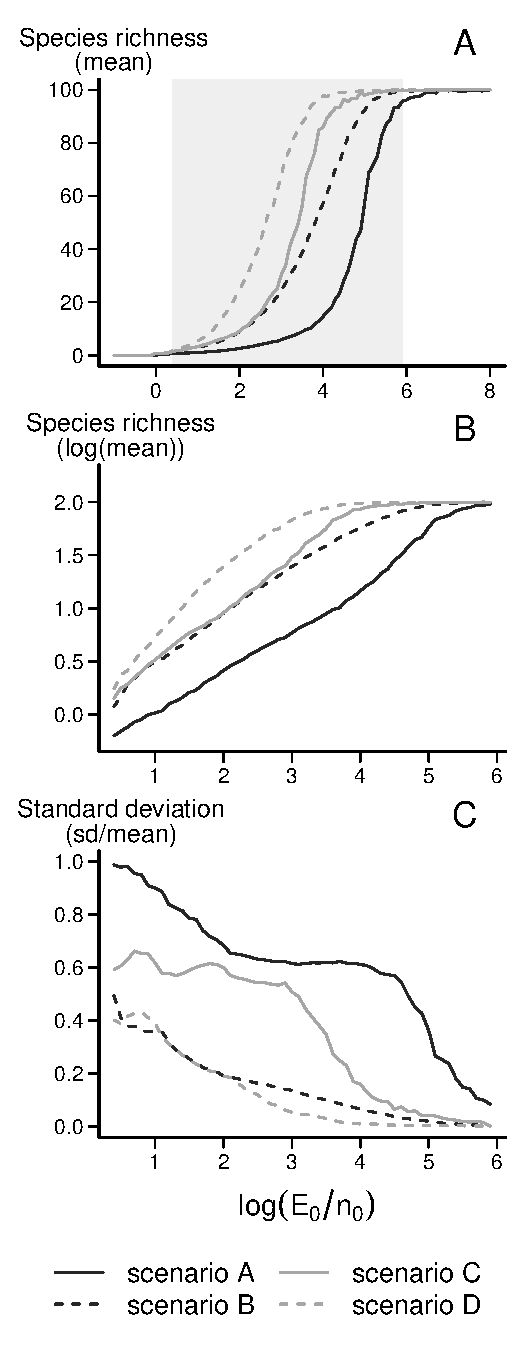
\includegraphics{chapitre4/fig/fig1.pdf}
\caption{\textbf{SAR and BAR} Cool}
\end{figure}

\begin{figure}[htbp]
\centering
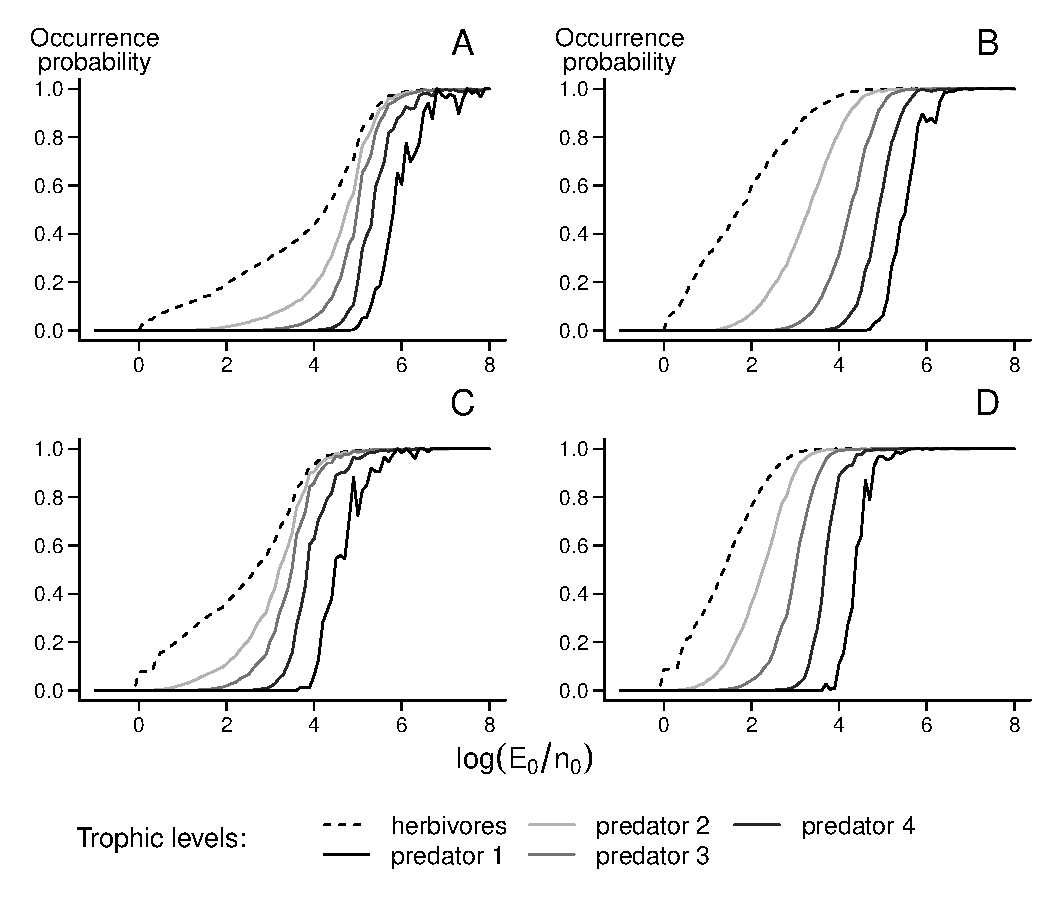
\includegraphics{chapitre4/fig/fig2.pdf}
\caption{\textbf{cool2} Cool}
\end{figure}

\begin{figure}[htbp]
\centering
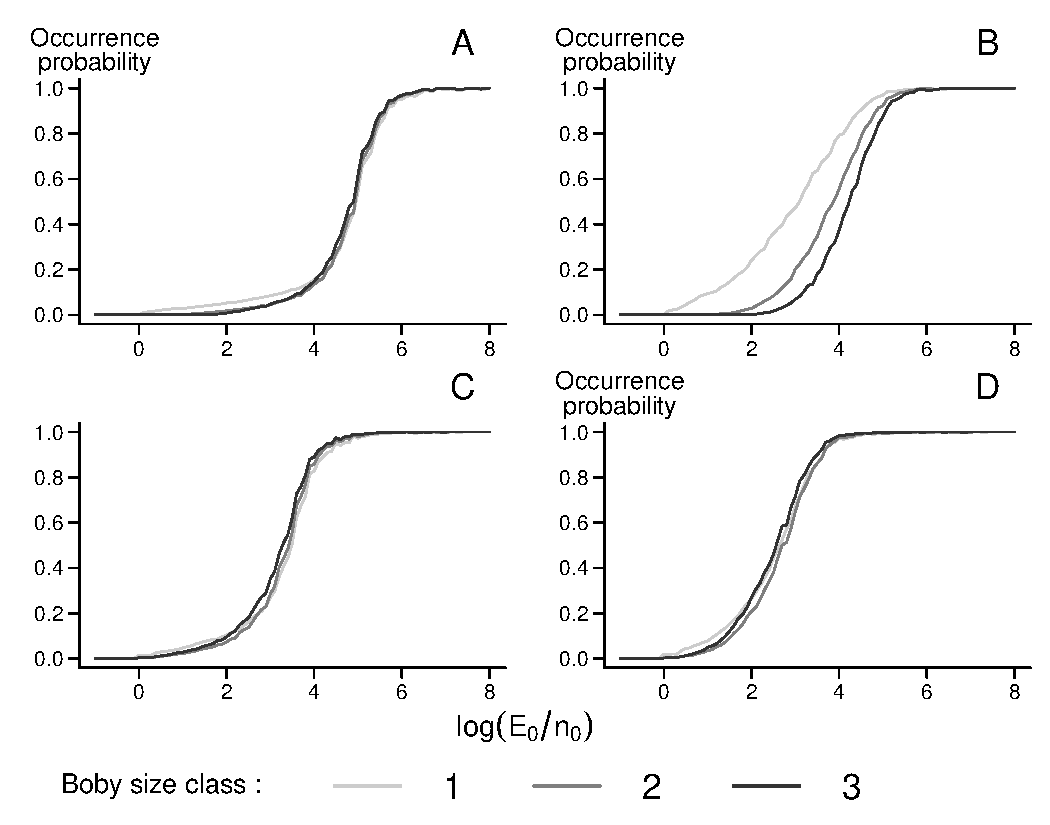
\includegraphics{chapitre4/fig/fig3.pdf}
\caption{\textbf{all} Cool}
\end{figure}

\begin{figure}[htbp]
\centering
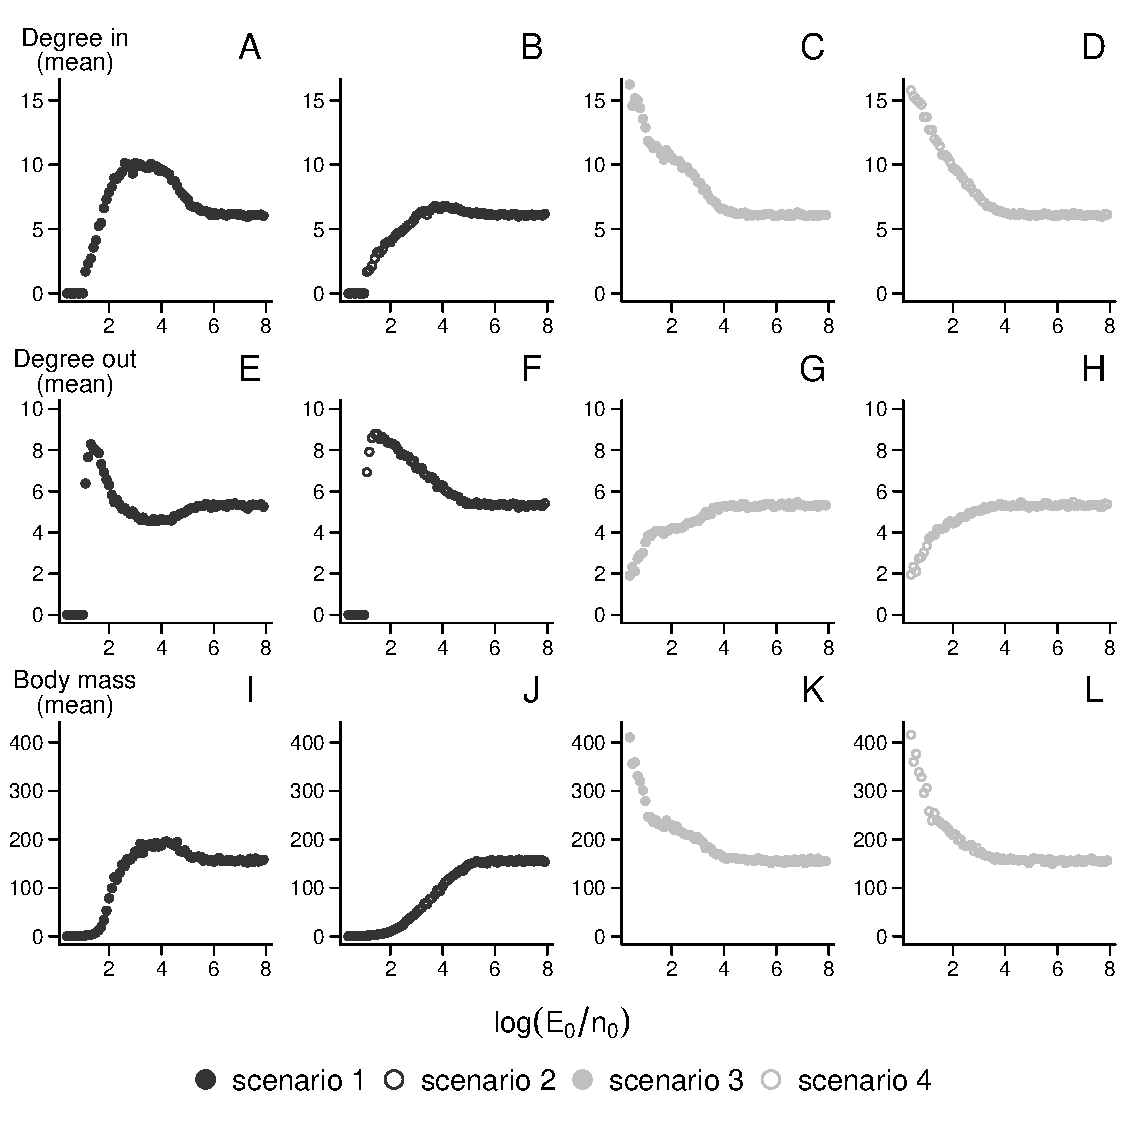
\includegraphics{chapitre4/fig/fig4.pdf}
\caption{\textbf{ols} Cool}
\end{figure}
